%begin detailed
\section{Основные понятия}
% overall documentation : frame 
\begin{frame}{Адгоритм Томпсона и НКА}
    \vspace{-5pt}
    \begin{block}{\bf Основные сведения}
        В информатике алгоритм построения Томпсона представляет собой метод преобразования регулярного выражения в эквивалентный недетерминированный конечный автомат (НКА). Этот НКА можно использовать для сопоставления строк с регулярным выражением.
        Регулярные выражения и недетерминированные конечные автоматы - это два представления формальных языков.
    \end{block}
\end{frame}% overall documentation

% descriptive documentation : frame 
\begin{frame}{Недетерминированные КА}\only<3> {\vspace{-5pt}}
    \vspace{-5pt}
    \only<1> {
        \begin{block}{\bf Определение}
            Недетерминированный конечный автомат (НКА) -- это детерминированный конечный автомат (ДКА), который не выполняет следующие условия:
            \begin{itemize}
                \item любой его переход единственным образом определяется по текущему состоянию и входному символу;
                \item чтение входного символа требуется для каждого изменения состояния.
            \end{itemize}
        \end{block}
    }
    \only<2> {
        \begin{block}{Определение}
            Недетерминированный конечный автомат (NFA) --- это пятёрка $\Aut\seq\langle Q,\Sigma, q_0, F, \delta \rangle${, где:
                    \begin{itemize}
                        \item $Q$ --- множество состояний;
                        \item $\Sigma$ --- алфавит терминалов;
                        \item $\delta$ --- множество правил перехода вида $\langle q_i, (a_i|\empt), M_i\rangle$, где $q_i\in Q$, $a_i\in \Sigma$, $M_i\in 2^Q$;
                        \item $q_0\in Q$ --- начальное состояние;
                        \item $F\subseteq Q$ --- множество конечных состояний.
                    \end{itemize}}
        \end{block}

        Сокращаем: $\langle q_1, a, q_2\rangle\in \delta\iff \langle q_1,a,M\rangle\in\delta\logand q_2\in M$.
    }
    \only<3> {
        \begin{wideitemize}
            \item $q \overset{\empt}{\longrightarrow} q'\iff (q=q')\logor\exists p_1,\dots,p_{k}(\langle q,\empt, p_1\rangle\in \delta\logand \langle p_k,\empt,q'\rangle\in\delta\logand\forall i,1\leq i<k\langle p_i,\empt,p_{i+1}\rangle\in\delta)$.

            \item $q\overset{a}{\longrightarrow}q'\iff \exists p,p'(q\overset{\empt}{\longrightarrow}p\logand \langle p, a, p'\rangle\in\delta\logand p'\overset{\empt}{\longrightarrow}q')$.

            \item $q \overset{a_1\dots a_k}{\longrightarrow} q'\iff \exists p_1,\dots,p_{k-1}(q\overset{a_1}{\longrightarrow}p_1\logand p_{k-1}\overset{a_k}{\longrightarrow}q'\logand \forall i,1\leq i<k-1(p_i\overset{a_{i+1}}{\longrightarrow}p_{i+1}))$.
        \end{wideitemize}

        \vspace{-5pt}
        \begin{block}{Определение}
            Язык $\Lang$, распознаваемый НКА $\Aut$ --- это множество слов $\bigl\lbrace{}w\mid\exists q\in F (q_0\transit{w}q)\bigr\rbrace{}$.
        \end{block}
    }
\end{frame} % descriptive documentation

\begin{frame}{Пример НКА}
    \vspace{-5pt}
    \begin{center}
        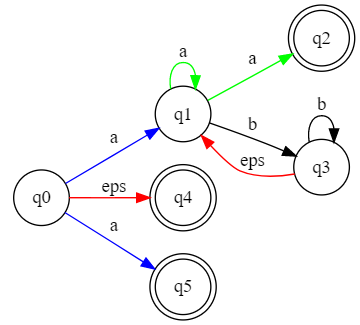
\includegraphics[width=3in, keepaspectratio]{images/thompson1.png} % the NFA example diagram placeholder
    \end{center}
\end{frame}% descriptive documentation
%end detailed


\section{Автомат Томпсона}
%begin detailed
% descriptive documentation : frame
\begin{frame}{Конструкция автомата Томпсона}\only<2> {\vspace{-5pt}}
    \vspace{-5pt}
    \begin{block}{\bf Алгоритм построения $\Thompson(r)$}
        \only<1-2>{Алгоритм работает рекурсивно, разбивая выражение на составляющие его подвыражения, из которых будет построен НКА с использованием набора правил. Точнее, из регулярного выражения $r$ полученный автомат $A$ с переходной функцией $\delta$ учитывает следующие свойства:}
        \begin{wideitemize}
            \only<1> {
                \item $A$ имеет ровно одно начальное состояние $q_{0}$, которое недоступно ни из какого другого состояния. То есть для любого состояния $q$ и любой буквы $a$ $\delta (q,a)$ не содержит $q_{0}$.
                \item $A$ имеет ровно одно конечное состояние $q_{f}$, которое недоступно ни из какого другого состояния. То есть для любой буквы $a$, $\delta (q_{f},a)=\emptyset$.
                \item Пусть $c$ - число конкатенаций регулярного выражения $r$, а $s$ — количество символов, не считая круглых скобок, то есть $\alter, \star, a, \empt$. Тогда число состояний $A$ равно 2$s - c$ (линейно по размеру $r$).
            } \only<2> {
                \item Число переходов, выходящих из любого состояния, не более двух.
                \item Поскольку НКА из $m$ состояний и не более $e$ переходов из каждого состояния может соответствовать строке длиной $n$ за время $O(emn)$, НКА Томпсона может выполнять сопоставление с образцом за линейное время, предполагая алфавит фиксированного размера.
            }
        \end{wideitemize}
    \end{block}
\end{frame} % descriptive documentation

\begin{frame}{Правила} \only<4> {\vspace{-5pt}}
    \vspace{-5pt}
    \only<1-4>{$N(s)$ и $N(t)$ являются NFA подвыражений $s$ и $t$ соответственно.}
    \only<1> {
        Пустое выражение $\empt$ преобразуется в

        \begin{tikzpicture}[>={Stealth[scale=1.2]},line join=bevel,scale=0.48]
            \tikzstyle{every node}+=[inner sep=0.3ex]
            \node (dummy) at (27.0bp,28.698bp) [draw,draw=none] {$\;\;\;$};
              \node (0) at (109.0bp,28.698bp) [draw,circle,fill=white, thick] {$\regexpstr{q}$};
              \node (1) at (200.7bp,28.698bp) [draw,circle, fill=white, double, double distance=1.5pt, thick] {$\regexpstr{f}$};
              \draw [->, thick] (dummy) ..controls (62.654bp,28.698bp) and (72.051bp,28.698bp)  .. (0);
              \draw [->, thick] (0) ..controls (137.06bp,28.698bp) and (149.67bp,28.698bp)  .. (1);
              \draw (149.5bp,36.198bp) node {$\empt$};
        \end{tikzpicture}
            

        Символ $a$ входного алфавита преобразуется в

        \begin{tikzpicture}[>={Stealth[scale=1.2]},line join=bevel,scale=0.48]
            \tikzstyle{every node}+=[inner sep=0.3ex]
            \node (dummy) at (27.0bp,28.698bp) [draw,draw=none] {$\;\;\;$};
              \node (0) at (109.0bp,28.698bp) [draw,circle,fill=white, thick] {$\regexpstr{q}$};
              \node (1) at (200.7bp,28.698bp) [draw,circle, fill=white, double, double distance=1.5pt, thick] {$\regexpstr{f}$};
              \draw [->, thick] (dummy) ..controls (62.654bp,28.698bp) and (72.051bp,28.698bp)  .. (0);
              \draw [->, thick] (0) ..controls (137.06bp,28.698bp) and (149.67bp,28.698bp)  .. (1);
              \draw (149.5bp,36.198bp) node {$\regexpstr{a}$};
        \end{tikzpicture}
    }
    \only<2> {
        Выражение объединения $s\alter t$ преобразуется в

        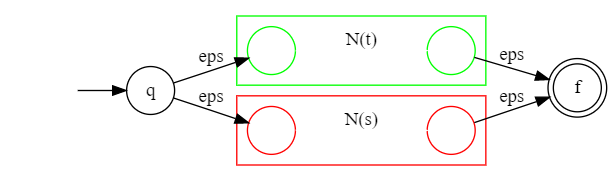
\includegraphics[width=4in, keepaspectratio]{images/thompson_rule1.png} % the Rule1 diagram placeholder

        Состояние $q$ переходит через $\empt$ либо в начальное состояние $N(s)$, либо $N(t)$. Их конечные состояния становятся промежуточными состояниями всего НКА и сливаются через два $\empt$-перехода в конечное состояние НКА.
    }
    \only<3> {
        Выражение конкатенации $st$ преобразуется в

        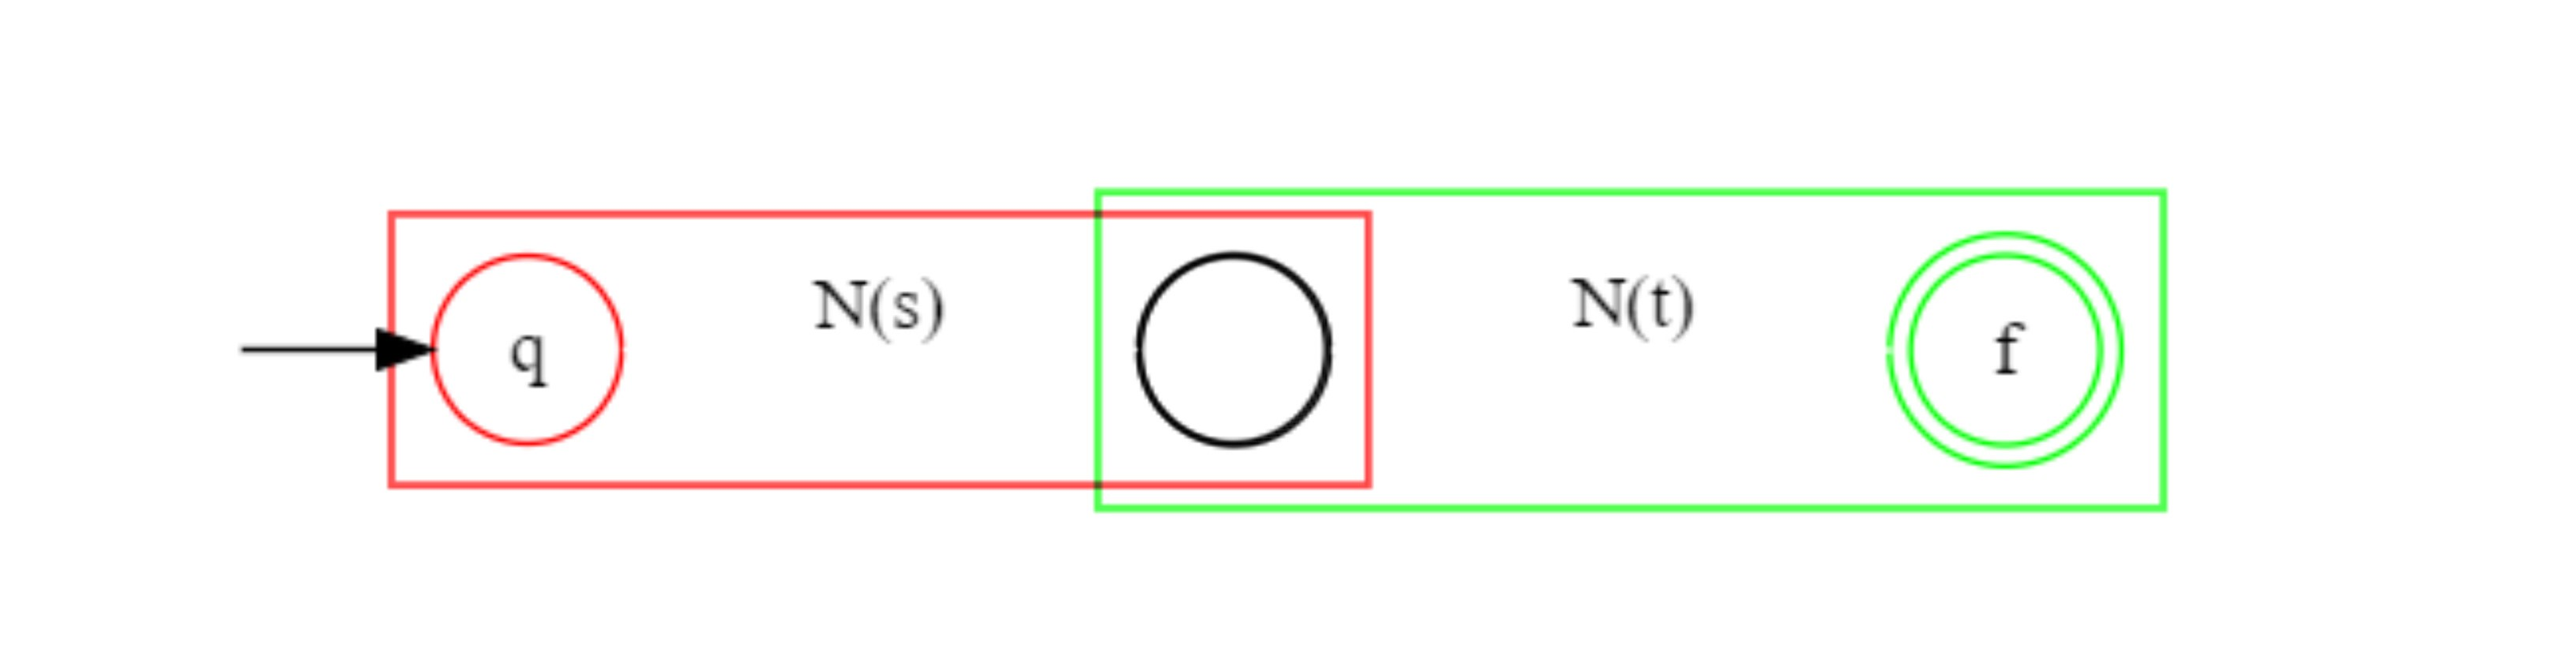
\includegraphics[width=4in, keepaspectratio]{images/thompson_rule2.png} % the Rule2 diagram placeholder

        Начальное состояние $N(s)$ является начальным состоянием всего НКА. Конечное состояние $N(s)$ становится начальным состоянием $N(t)$. Конечное состояние $N(t)$ является конечным состоянием всего НКА.
    }
    \only<4> {
        Выражение Клини Стар $s\star$ преобразуется в

        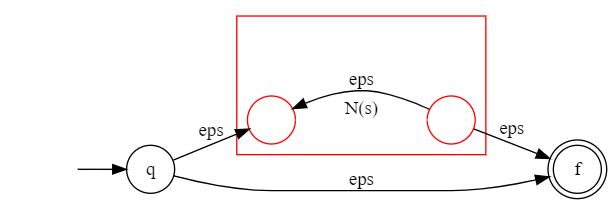
\includegraphics[width=4in, keepaspectratio]{images/thompson_rule3.png} % the Rule3 diagram placeholder

        $\empt$-переход соединяет начальное и конечное состояние НКА с промежуточным НКА $N(s)$. Другой $\empt$-переход от внутреннего конечного к внутреннему начальному состоянию $N(s)$ допускает повторение выражения $s$ в соответствии с оператором $\star$.

        Заключенное в скобки выражение (выражения) преобразуется в само $N(s)$.
    }
\end{frame}% descriptive documentation
%end detailed

\begin{frame}{Построение $\Thompson\TypeIs\RegexTYPE\to\NFATYPE$}
	Регулярное выражение:
	%template_oldregex

	Автомат:

	%template_result

\end{frame}

%begin detailed
% overall documentation : section 
\section{Обсуждение}
\begin{frame}{Cвойства автомата Томпсона}
    \begin{itemize}
        \item Единственное начальное состояние
        \item Единственное конечное состояние
        \item Не больше двух переходов из каждого состояния
    \end{itemize}
\end{frame}
%end detailed